% Budget: ~2.75 pages (1.5 quality + 1.25 performance).
% Numbers in Tables II-III come from results/*_indicators.csv (30 runs x 500 gens,
% restart fix included) and results/tune_qiea_restart_confirm_*.csv (20 seeds).
% Significance: two-sided Mann-Whitney U with Holm correction over the four
% QIEA-vs-baseline comparisons per instance (runs of different algorithms are
% independent, so an unpaired test is used; the paired Wilcoxon used in logs.txt
% gives the same conclusions everywhere).
\section{Experimental Evaluation}
\label{sec:experiments}

\subsection{Setup}
HQIEA-ARGC is compared with NSGA-II~\cite{deb2002nsga2}, SPEA2~\cite{zitzler2001spea2},
MOEA/D~\cite{zhang2007moead} and RVEA~\cite{cheng2016rvea}, all from
pymoo~0.6.2~\cite{blank2020pymoo}. The baselines search the same permutation space
with permutation-valid operators: random-permutation initialization, order
crossover, and inversion mutation. MOEA/D and RVEA use the same $H=126$ weight
vectors as HQIEA-ARGC (MOEA/D with 15 neighbors and neighbor-mating probability
0.9); NSGA-II and SPEA2 use a population of 80. All five algorithms call the same
evaluation function, so they optimize an identical problem. Each algorithm runs
30 times per instance for 500 generations, with seeds $0,\dots,29$. The
population sizes of NSGA-II and SPEA2 (80) differ from the other three (126); in a
separate study that scaled the population of all five algorithms together from
35 to 495, HQIEA-ARGC's relative standing did not change significantly. HQIEA-ARGC
went through the tuning study described in \cref{sec:algorithm}, whereas the
baselines use pymoo's default settings, so any tuning advantage favors
HQIEA-ARGC. The quality runs used Python~3.12, NumPy~2.5.2 and pymoo~0.6.2 on the
machine described in \cref{sec:parallel}.

No true Pareto front is known for these instances, so we measure solution quality
by hypervolume (HV), with spacing and spread as secondary indicators. For each
instance, one reference point, $1.1\times$ the component-wise maximum over all
final fronts of all algorithms and runs, is shared by every run. A Kruskal--Wallis
test checks whether the five algorithms differ on an instance. Each
HQIEA-ARGC--baseline pair is then compared with a two-sided Mann--Whitney $U$ test,
with a Holm correction over the four comparisons per instance.

\subsection{Solution quality}
\Cref{tab:hv} reports each algorithm's mean HV relative to the best algorithm on
that instance. The five algorithms differ significantly on every instance
(Kruskal--Wallis $p<10^{-16}$). No single baseline dominates: SPEA2 and RVEA lead
on the small CVRPLIB instances, and MOEA/D and RVEA on the larger ones and on all
three Sibiu routes. HQIEA-ARGC ranks last on all seven instances, at 30--58\% of
the best algorithm's HV. Of its 28 pairwise comparisons, 27 favor the baseline
significantly. The one exception is route1\_334, the largest instance, where
HQIEA-ARGC reaches 94\% of NSGA-II's HV and the difference is not significant
($p=0.19$). The gap is largest against MOEA/D and RVEA, which reach 1.5 to 3.3
times HQIEA-ARGC's HV on every instance.

HQIEA-ARGC returns 7--25 non-dominated solutions on average, against 53--80
for NSGA-II and SPEA2 and 63--123 for MOEA/D, and has larger spacing values
(106--404 vs.\ 20--75 for NSGA-II and SPEA2). Front size alone does not explain
the HV gap, however: RVEA returns similarly small fronts (16--23 solutions) and
still achieves the best HV on four instances.

\begin{table}[t]
\centering
\caption{Mean hypervolume relative to the best algorithm per instance (1.000 =
best; 30 runs, 500 generations; HQIEA = HQIEA-ARGC). $^\dagger$: HQIEA-ARGC vs.\ NSGA-II not
significant ($p=0.19$); all other HQIEA-ARGC comparisons $p<0.01$ (Mann--Whitney,
Holm).}
\label{tab:hv}
\setlength{\tabcolsep}{4pt}
\begin{tabular}{@{}lrrrrr@{}}
\toprule
Instance & HQIEA & NSGA-II & SPEA2 & MOEA/D & RVEA \\
\midrule
A-n32-k5    & 0.571 & 0.989 & 0.992 & 0.876 & \textbf{1.000} \\
A-n33-k5    & 0.541 & 0.956 & \textbf{1.000} & 0.840 & 0.994 \\
E-n101-k8   & 0.300 & 0.478 & 0.542 & 0.978 & \textbf{1.000} \\
M-n200-k16  & 0.330 & 0.368 & 0.429 & \textbf{1.000} & 0.928 \\
route2\_199 & 0.581 & 0.748 & 0.815 & 0.987 & \textbf{1.000} \\
route3\_202 & 0.489 & 0.660 & 0.720 & 0.902 & \textbf{1.000} \\
route1\_334 & 0.577$^\dagger$ & 0.614 & 0.691 & \textbf{1.000} & 0.927 \\
\bottomrule
\end{tabular}
\end{table}

\subsection{Diagnosis: plateau and restart correction}
Before the restart was added, HQIEA-ARGC's HV was only 17--45\% of the best
algorithm's on every instance. To see why, we traced HV every 10 generations for
all algorithms, with and without the restart, on a small, a medium and a large
instance (3 seeds each, reference point fixed per run; \cref{fig:trace}).
Without the restart, HQIEA-ARGC is competitive with the baselines for the first
50--100 generations on A-n32-k5, but on all three instances its HV eventually
stops improving (no gain above 0.5\% of its final value) from generation 60--150
on A-n32-k5 and 410--450 on route2\_199, while every baseline keeps improving
until generation 500. On route1\_334 the plateau had not yet been reached at
generation 500, but progress had slowed. The ARGC trigger, meant for exactly this
situation, stays inactive (\cref{sec:algorithm}). With the restart, HQIEA-ARGC
continues to improve until the end of the run on all three instances, and its
final HV is 16--68\% higher than without it on the same seed.

\begin{figure*}[t]
\centering
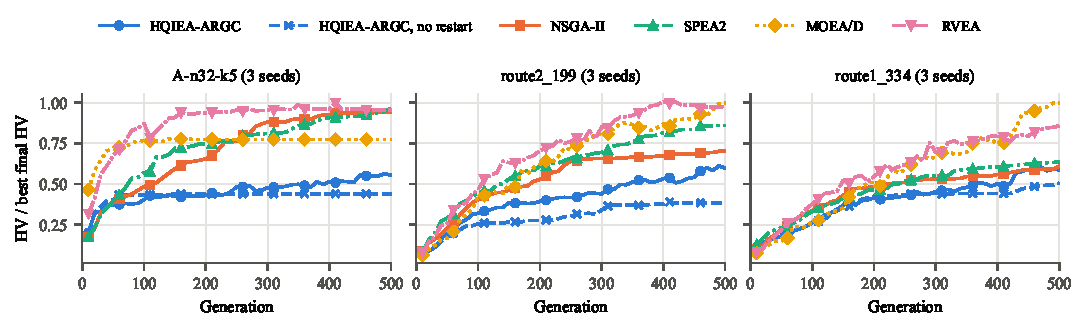
\includegraphics[width=\textwidth]{figures/trace_restart.pdf}
\caption{Hypervolume vs.\ generation, relative to the best final HV of any
algorithm in the same run (median over 3 seeds). Without the restart (dashed),
HQIEA-ARGC stops improving early on A-n32-k5 and late on route2\_199; with the
restart (solid) it keeps improving, but stays below the baselines.}
\label{fig:trace}
\end{figure*}

\Cref{tab:restart} isolates the restart's effect. With seeds matched, so that both
variants start from the same initial population, the restart increases HV
significantly on all seven instances, by 28--66\%. It is the only change in our
tuning study that was significant on every instance in the same direction. It
narrows HQIEA-ARGC's gap to the best algorithm by roughly half, from 17--45\% to
30--58\% of the best HV, but does not close it.

\begin{table}[t]
\centering
\caption{Effect of the plateau-gated restart: HQIEA-ARGC mean HV with vs.\
without restart (20 seeds, 500 generations, paired Wilcoxon on matched seeds).}
\label{tab:restart}
\begin{tabular}{@{}lrr@{}}
\toprule
Instance & HV change & $p$ \\
\midrule
A-n32-k5    & $+29.7\%$ & $3.7\times10^{-3}$ \\
A-n33-k5    & $+32.0\%$ & $1.3\times10^{-4}$ \\
E-n101-k8   & $+66.0\%$ & $1.9\times10^{-6}$ \\
M-n200-k16  & $+35.4\%$ & $2.6\times10^{-4}$ \\
route2\_199 & $+36.1\%$ & $6.3\times10^{-5}$ \\
route3\_202 & $+40.4\%$ & $1.9\times10^{-6}$ \\
route1\_334 & $+27.7\%$ & $2.1\times10^{-4}$ \\
\bottomrule
\end{tabular}
\end{table}

Several other levers did not explain the remaining gap. Tuning the neighborhood
size $|B(i)|$, making ARGC fire more often, changing its boost magnitude, and scaling
the population size $H$ jointly for all five algorithms (35 to 495) either had no
significant effect or made HV worse. Promising 5-seed screens repeatedly failed
15-seed confirmation, so we changed a default only after a confirmation run.

\subsection{Runtime and parallel performance}
% TODO: depends on the performance work (submission2.txt sections 7-8).
% (The runtime-breakdown table is already in Sec. parallel, tab:profile.)
% - Serial optimization results (vectorized Tchebycheff, Numba evaluator).
% - Speedup/efficiency vs workers, multiprocessing vs Numba threads, P/E cores.
% - Time-to-quality: HV vs wall-clock for all five algorithms.
% Hardware: Intel Core i7-12700H (6 P-cores + 8 E-cores, 20 threads), 62 GiB,
% Python 3.12, NumPy 2.5.2, pymoo 0.6.2, BLAS pinned to 1 thread per process.
